\chapter{Hypothesis Testing based on Normal Distribution}

\section{Null and Alternative Hypotheses}

\begin{definition}[Statistical Hypothesis]
A statistical hypothesis is an assertion or conjecture concerning one or more populations
\end{definition}
{\color{blue}It is important to understand that the rejection of a hypothesis is to conclude that it is false, while the acceptance of a hypothesis merely implies that we have insufficient evidence to believe otherwise. Because of this terminology, the statistician or experimenter will often chose to state the hypothesis in a form that will hopefully be rejected.}
\begin{definition}[Null Hypothesis]
Hypothesis that we formulate with the hope of rejecting, denoted by $H_0$. A null hypothesis concerning a population parameter will always be stated to specify an exact value of the parameter
\end{definition}
\begin{definition}[Alternative Hypothesis]
The rejection of $H_0$ leads to the acceptance of an alternative hypothesis, denoted by $H_1$. It allows for the possibility of several values.
\end{definition}
For example, if we wish to determine whether the mean IQ of the pupils of a certain school is different from 100, we could set $H_0: \mu =  100$ against $H_1: \mu \neq 100$. This is called a two-sided alternative. The test is called a two-sided (or two-tailed) test. We may like to test whether the mean IQ of the pupils is greater than 100 (or less than 100). This is called a one-sided alternative and the test is called a one-sided (or one-tailed) test. That is, $H_0: \mu = 100$ against $H_1: \mu > 100$ or $H_0: \mu = 100$ against $H_1: \mu < 100$. \\
The procedure for statistical inference is quite simple. We choose a random sample and calculate the sample parameter. Then, we calculate how likely it was possible to obtain a value that was as favourable to our alternative hypothesis assuming that the null hypothesis was true. If the probability of this occurring is low, then we can reject the null hypothesis. Typically, we set the value of statistical significance at $5\%$. That is, if the probability of obtaining such a result (or more favourable is less than $5\%$, we can reject the null hypothesis. \\
The whole framework of hypothesis testing is to look for evidence to reject the null hypothesis. (Instead, if the framework was to find evidence to reject the alternative hypothesis and you were not able to find such evidence, you might conclude that the alternative hypothesis is true. But others may argue that you simply did not dig deep enough for evidence.) 
\begin{note}
\end{note}
It is worth understanding the difference between "accept" and "do not reject" in statistics. There are only two kinds of theories in the world - false theories, and theories that are yet to be proved false. For example, you hypothesise that there are no black swans on Earth. Obviously if you see a single black swan, your hypothesis immediately fails. On the other hand, if you don't see any black swan for 10 years, you still cannot be sure that there is no black swan (someone may argue that you did not search hard enough). In this sense, we can say that we do not have sufficient evidence to reject the hypothesis that there are no black swans on Earth (however, we have not yet established its truth). \\
Hence, we set our null hypothesis to be the status quo (what is currently believed) and pit it against our alternative hypothesis (what we wish to establish).
\begin{note}
\end{note}
By convention (and theoretically supported), we usually write the null hypothesis in the "equal" form, i.e., $H_0: \theta = \theta_0$, with $\theta_0$ being a fixed constant. So the hypotheses have three possible forms:
\begin{itemize}
    \item $H_0: \theta = \theta_0$ versus $H_0: \theta > \theta_0$; in this case $H_0: \theta = \theta_0$ in fact means $\theta \leq \theta_0$
    \item $H_0: \theta = \theta_0$ versus $H_0: \theta < \theta_0$; in this case $H_0: \theta = \theta_0$ in fact means $\theta \geq \theta_0$
    \item $H_0: \theta = \theta_0$ versus $H_1: \theta \neq \theta_0$
\end{itemize}
So, we need to check the form of $H_1$ to ensure the meaning of $H_0: \theta = \theta_0$ in practice.
\subsection{Types of Error}
There are two possible true answers (we call it the state of nature) which we don't know, i.e., we don't know if $H_0$ is true or $H_1$ is true.\\
\begin{figure}[ht]
    \centering
    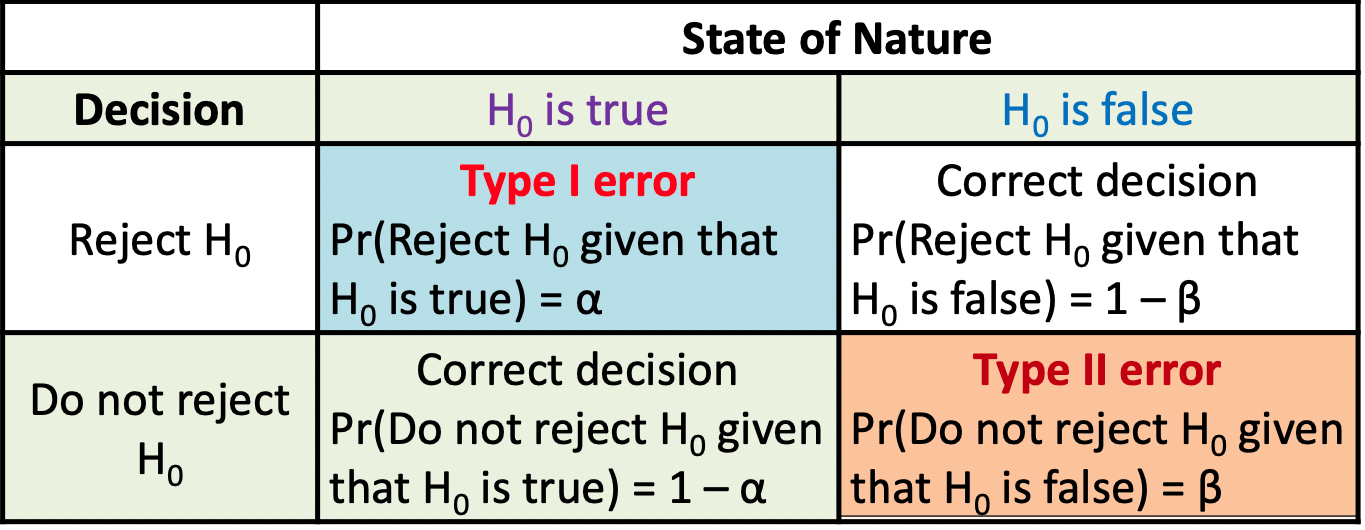
\includegraphics[width = 14cm]{Images/Types of Error.png}
    \caption{Types of Error}
    \label{fig:my_label}
\end{figure}
A \textbf{Type I} error is when you reject $H_0$ even when $H_0$ is actually true. It is considered a serious type of error. Many statisticians and experimenters fabricate data just to be able to reject the null hypothesis (and persuade people that their theory is correct). \\
A \textbf{Type II} error is not rejecting $H_0$ when $H_0$ is false. When we say that $H_0$ is false, we actually mean that $H_1$ is true. \\
Here, $\alpha$ is the level of significance. $\alpha$ is equal to the probability of making a type I error, i.e., the probability of rejecting $H_0$ even when it is true. Formally, $\alpha = P($reject $H_0|H_0$ is true$)$. \\
$\alpha$ is set by the researcher in advance (it is usually set at $5\%$ or $1\%$). \\
$\beta$ is the probability of committing a type II error, i.e., the probability of not rejecting $H_0$ even when $H_0$ is false. Formally, $\beta$ = $P($do not reject $H_0|H_1)$. \\
$$
1 - \beta = \textbf{Power of a test} = P(\textit{reject }H_0|H_1)
$$
{\color{blue} Note that it is not possible to determine the probability of committing a type II error, denoted by $\beta$, unless we have a specific alternative hypothesis.} \\
\begin{note}
\end{note}
Type I error is usually treated more seriously (since it causes a change in the status quo); so we need to control it in the first place. We set a significance level, called $\alpha$, and require that the decision rule satisfy $P($reject $H_0|H_0$ is true$) \leq \alpha$. Once we have controlled our type I error (upper bound it), we try to minimize type II error (so that our test is powerful) and so, we typically require  $P($reject $H_0|H_0$ is true$) = \alpha$. This is so that the type I error is controlled but maximized (up to an acceptable level) to reduce the type II error. Notice that when establishing a testing rule, type I and type II errors trade off each other. This similar to the trade-off between the confidence level and the width of a confidence interval - it is possible to gain confidence by expanding our interval but then it becomes meaningless. For example, if you set $\alpha = 0.0001$, i.e., your chances of making a type I error is $0.01\%$ but then your decision rule will commit a type II error with large probability.
\begin{note}
\end{note}
Observe that when a test is performed, one can make at most one type of error since if $H_0$ is rejected, type I error is possible and if $H_0$ is not rejected, then type II error is possible. These are disjoint events. 
\begin{note}
\end{note}
Hypothesis testing cannot be used to determine the truth value of any statement. It is a decision making process. Even if you reject the null hypothesis, it does not mean that the null hypothesis is false. It simply means that the evidence suggested that it was unlikely for the null hypothesis to be true. In any case, you might have made an error (which you will not find out until new evidence comes to light).
\begin{note}
\end{note}
{\color{blue}The hypotheses should not contain any random variables since it must be a statement with a fixed truth value. For example, $H_0: \bar{X} < 10$ is not a valid null hypothesis.}
\begin{note}
\end{note}
Statistical significance refers to the claim that a result from data generated by testing or experimentation is not likely to occur randomly or by chance but is instead likely to be attributable to a specific cause. A p-value less than 0.05 is statistically significant. It indicates strong evidence against the null hypothesis, as there is less than a 5$\%$ probability the null is correct (and the results are random). Therefore, we reject the null hypothesis, and accept the alternative hypothesis.
\subsection{Acceptance and Rejection Regions}
To test a hypothesis about a population parameter, we first select a suitable test statistic for the parameter under hypothesis. Once the significance level, $\alpha$, is given, a decision rule can be found such that it divides the set of all possible values of the test statistic into 2 regions, one being the rejection region (or critical region) and the other the acceptance region. \\
Once a sample is taken, the value of the test statistic is obtained. If the test statistic assumes a value in the rejection region, the null hypothesis is rejected; otherwise it is not rejected. \\
The value that separates the rejection and acceptance regions is called the critical value.

\section{Hypothesis Testing Concerning Mean}
\subsection{Known Variance}
Consider the problem of testing the hypothesis concerning the mean, $\mu$, of a population with:
\begin{enumerate}
    \item Variance, $\sigma^2$, known
    \item Underlying distribution is normal or $n$ is sufficiently large (say $n > 30$)
\end{enumerate}
\subsubsection{Two-sided Test}
Test $H_0: \mu = \mu_0$ against $H_1: \mu \neq \mu_0$. \\
When the population is normal or the sample size is large (then by the central limit theorem), we can expect that $\bar{X} \sim N\left(\mu, \dfrac{\sigma^2}{n}\right)$. Hence under $H_0: \mu = \mu_0$, we have $\bar{X} \sim N\left(\mu_0, \dfrac{\sigma^2}{n}\right)$. \\
\textbf{Critical Value Approach} \\
By using a significance level of $\alpha$, it is possible to find two critical values $\bar{x_1}$ and $\bar{x_2}$ such that the interval $\bar{x_1} < \bar{X} < \bar{x_2}$ defines the acceptance region and the two tails of the distribution $\bar{X} < \bar{x_1}$ and $\bar{X} > \bar{x_2}$ constitute the critical (or rejection region). Hence, in this case there are two cut-off values (critical values), defining the regions of rejection and acceptance. (Observe that the acceptance and rejection regions are mutually exclusive and exhaustive. This ensures that we make one of two decisions: reject $H_0$ or do not reject $H_0$.) \\
\begin{figure}[ht]
    \centering
    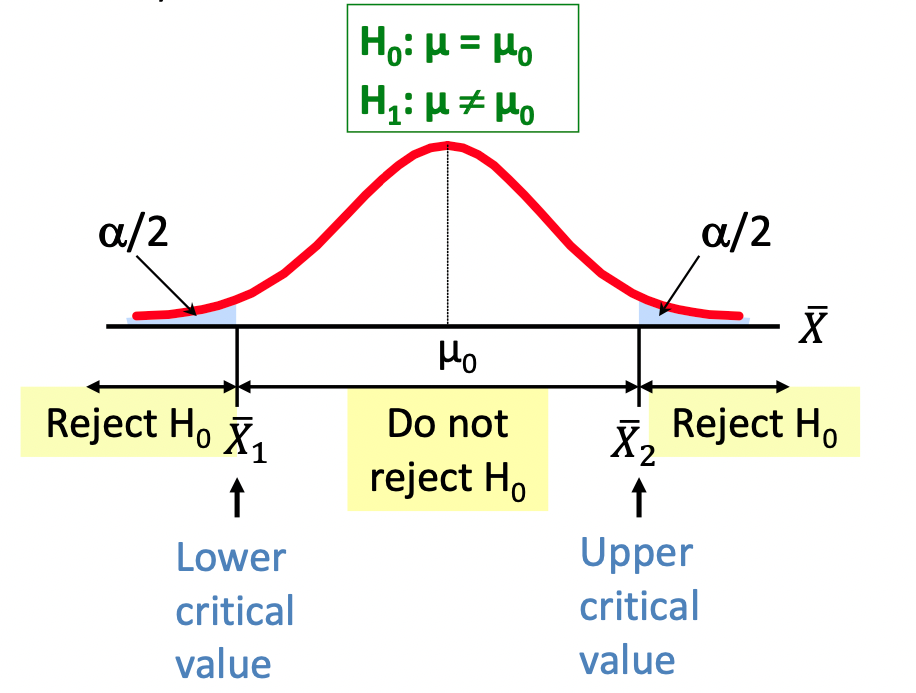
\includegraphics[width = 14cm]{Images/Two-sided test.png}
    \caption{Two-sided test}
    \label{fig:my_label}
\end{figure}
The critical region can be given in terms of z values by means of the transformation $Z = \dfrac{\bar{X} - \mu_0}{\sigma/\sqrt{n}} \sim N(0,1)$ (Note that $\mu_0$ is the value of $\mu$ under $H_0$). \\
Therefore,
$$
P\left( -z_{\alpha/2} < \dfrac{\bar{X} - \mu_0}{\sigma/\sqrt{n}} < z_{\alpha/2}
\right) = 1 - \alpha
$$
or
$$
P\left( \mu_0 -z_{\alpha/2}\dfrac{\sigma}{\sqrt{n}} < \bar{X} < \mu_0 + z_{\alpha/2}\dfrac{\sigma}{\sqrt{n}}
\right) = 1 - \alpha
$$
Hence, $\bar{x_1} =\mu_0 -z_{\alpha/2}\dfrac{\sigma}{\sqrt{n}} $ and $\bar{x_2} = \mu_0 + z_{\alpha/2}\dfrac{\sigma}{\sqrt{n}}$
From the population, we select a random sample of size $n$ and compute the sample mean. If $\bar{X}$ falls in the acceptance region $\bar{x_1} < \bar{X} < \bar{x_2}$, we conclude that $\mu = \mu_0$; otherwise we reject $H_0$ and accept that $H_1: \mu \neq \mu_0$. \\
Since $Z = \dfrac{\bar{X} - \mu_0}{\sigma/\sqrt{n}}$, therefore  $\bar{x_1} < \bar{X} < \bar{x_2}$ is equivalent to $-z_{\alpha/2} < Z < z_{\alpha/2}$. The critical region is usually stated in terms of $Z$ rather than $\bar{X}$.
\subsubsection{Relationship between two-sided test and Confidence Interval}
The two-sided test procedure just described is equivalent to finding a $(1 - \alpha)100\%$ confidence interval for $\mu$. Then, $H_0$ is accepted if the confidence interval covers $\mu_0$. If the C.I. does not cover $\mu_0$, we reject $H_0$ in favour of the alternative $H_1: \mu \neq \mu_0$ since
$$
P\left( \mu -z_{\alpha/2}\dfrac{\sigma}{\sqrt{n}} < \bar{X} < \mu + z_{\alpha/2}\dfrac{\sigma}{\sqrt{n}}
\right) = 1 - \alpha \iff P\left( \bar{X} -z_{\alpha/2}\dfrac{\sigma}{\sqrt{n}} < \mu < \bar{X} + z_{\alpha/2}\dfrac{\sigma}{\sqrt{n}}
\right) = 1 - \alpha 
$$
\begin{note}
\end{note}
{\color{blue}Confidence interval is equivalent to the hypothesis testing if, and only if, the latter is two-sided; this is applicable not only for the mean related inference but also for the variance related inference.}
\subsubsection{p-value Approach to Testing}
\begin{definition}[p-value]
p-value is defined as the probability of obtaining a test statistic more extreme (in favour of the alternative hypothesis) ($\leq$ or $\geq$) than the observed sample given the $H_0$ is true. It is also called the observed level of significance.
\end{definition}
\begin{enumerate}
    \item Convert a sample statistic to a test statistic
    \item Obtain the p-value
    \item Compare the p-value with $\alpha$. If p-value < $\alpha$, reject $H_0$. If p-value $\geq \alpha$, do not reject $H_0$.
\end{enumerate}
\begin{note}
\end{note}
Using p-value or the rejection region approach to perform the test must result in exactly the same conclusion/decision in terms of reject or do not reject $H_0$. \\
That is, p-value $ < \alpha \iff$ the test statistic is in the rejection region.
\begin{note}
\end{note}
\imp{To get the p-value for a two-sided test, 
\begin{enumerate}
    \item Take the minimum of the probability of obtaining a test statistic larger than observed value, and lower than observed value (because you don't know which is actually true: $\theta > \theta_0$ or $\theta < \theta_0$. So the more extreme one will have lower probability. Also, exactly one of $\theta > \theta_0$ or $\theta < \theta_0$ is true if the alternative hypothesis is true).
    \item Multiply this by 2 to get the p-value.
\end{enumerate}
}
\subsubsection{One-sided Test}
(a) Test $H_0: \mu = \mu_0$ against $H_1: \mu > \mu_0$. \\
Let $Z = \dfrac{\bar{X} - \mu }{\sigma/\sqrt{n}}$. Then, $H_0$ is rejected if the observed values of $Z$, say $z$, is greater than $z_{\alpha}$. Note that there is only one critical value since the rejection area is only one tail (in this case, the upper tail of the distribution).\\
(b) Test $H_0: \mu = \mu_0$ against $H_1: \mu < \mu_0$. \\
Let $Z = \dfrac{\bar{X} - \mu }{\sigma/\sqrt{n}}$. Then, $H_0$ is rejected if the observed values of $Z$, say $z$, is greater than $-z_{\alpha}$. Note that there is only one critical value since the rejection area is only one tail (in this case, the lower tail of the distribution).
\subsection{Unknown Variance}
Consider the problem of testing the hypothesis concerning the mean, $\mu$, of a population with:
\begin{enumerate}
    \item Variance unknown
    \item Underlying distribution is normal
\end{enumerate}
(1) Two-sided Test \\
 Test $H_0: \mu = \mu_0$ against $H_1: \mu \neq \mu_0$. 
 Let $T = \dfrac{\bar{X} - \mu_0}{S/\sqrt{n}}$ where $S^2$ is the sample variance. Then, $H_0$ is rejected if the observed value of $T$, say $t$, $ > t_{n - 1; \alpha/2}$ or $ < -t_{n - 1; \alpha/2}$. \\
 (2) One-sided Test \\
 Test $H_0: \mu = \mu_0$ against $H_1: \mu > \mu_0$.
 Then $H_0$ is rejected if $t > t_{n - 1; \alpha}$
 Test $H_0: \mu = \mu_0$ against $H_1: \mu < \mu_0$.
  Then $H_0$ is rejected if $t < -t_{n - 1; \alpha}$
\section{Hypotheses Testing Concerning Difference Between 2 Means}
\subsection{Known Variances}
\begin{enumerate}
    \item Variances $\sigma_1^2$ and $\sigma_2^2$ are known
     \item Underlying distributions are normal or both $n_1$ and $n_2$ are sufficiently large (greater than 30)
\end{enumerate}
We know that the difference of two normal distributions follows a normal distribution. Then, we can proceed as before using the concepts of p-value or acceptance/rejection regions.
\subsection{Large Sample Testing with Unknown Variances}
\begin{enumerate}
    \item Variances $\sigma_1^2$ and $\sigma_2^2$ are unknown
     \item Both $n_1$ and $n_2$ are sufficiently large (greater than 30)
\end{enumerate}
\subsection{Unknown but Equal Variances}
\begin{enumerate}
    \item Variances $\sigma_1^2$ and $\sigma_2^2$ are unknown but equal
     \item Both $n_1$ and $n_2$ are small (less than 30)
\end{enumerate}
\subsection{Paired Data}
\section{Hypothesis Testing Concerning Variance}
\subsection{One Variance Case}
Assume that the underlying distribution is normal. Let $X_1, X_2, \dots, X_n$ be a random sample of size $n$ drawn from a (approximate) $N(\mu, \sigma^2)$ distribution, where $\sigma^2$ is unknown. \\
We wish to test the null hypothesis $H_0: \sigma^2 = \sigma_0^2$. We know that $\chi^2 = \dfrac{(n - 1)S^2}{\sigma_0^2} \sim \chi^2(n-1)$. \\
Hence $H_0: \sigma^2 = \sigma_0^2$ is rejected if the observed $\chi^2$-value lies in the critical region (here, our test statistic is $\dfrac{(n - 1)S^2}{\sigma_0^2}$). The critical region depends on the alternative hypothesis, and is summarised as follows:
\renewcommand{\arraystretch}{1.5}
\begin{table}[h]
    \centering
    \begin{tabular}{|c|c|}
    \hline
      \textbf{$H_1$}   &  \textbf{Critical Region} \\
      \hline
        $\sigma^2 > \sigma_0^2$ & $\chi^2 > \chi_{n - 1; \alpha}^2$ \\
      \hline
        $\sigma^2 < \sigma_0^2$ &  $\chi^2 < \chi_{n - 1; 1- \alpha}^2$\\
      \hline
        $\sigma^2 \neq \sigma_0^2$ & $\chi^2 < \chi_{n - 1; 1- \alpha/2}^2$ or $\chi^2 > \chi_{n - 1; \alpha/2}^2$ \\
      \hline
    \end{tabular}
    \caption{Critical Regions for Different Alternative Hypotheses}
    \label{tab:my_label}
\end{table}
where $P(W > \chi_{n - 1; \alpha}^2) = \alpha$ with $W \sim \chi^2(n-1)$
\subsection{Ratio of Variances}
Let us assume that the underlying distribution is normal and the means are unknown.
When we are comparing the precision of one measuring device with that of another, or the variability in grading practices of one teacher with that of another, or the consistence of one production process with that of another, we are testing about the comparison between two population variances (or standard deviations). \\
We know that when two independent samples of sizes $n_1$ and $n_2$ are randomly selected from two normal populations, then $F = \dfrac{S_1^2/\sigma_1^2}{S_2^2/\sigma_2^2} \sim F(n_1 - 1, n_2 - 1)$. Under $H_0: \sigma_1^2 = \sigma_2^2$, $F = \dfrac{S_1^2}{S_2^2} \sim F(n_1 - 1, n_2 - 1)$. \\
Our test statistic is $F = \dfrac{S_1^2}{S_2^2}$. Hence $H_0: \sigma_1^2 = \sigma_2^2$ is rejected if the observed F-value lies in the critical region . The critical region depends on the alternative hypothesis, and is summarised as follows:
\renewcommand{\arraystretch}{1.5}
\begin{table}[h]
    \centering
    \begin{tabular}{|c|c|}
    \hline
      \textbf{$H_1$}   &  \textbf{Critical Region} \\
      \hline
        $\sigma_1^2 > \sigma_2^2$ & $F > F_{n_1 - 1, n_2 - 1; \alpha}$ \\
      \hline
        $\sigma_1^2 < \sigma_2^2$ & $F < F_{n_1 - 1, n_2 - 1; 1 - \alpha}$ \\
      \hline
        $\sigma_1^2 \neq \sigma_2^2$ & $F < F_{n_1 - 1, n_2 - 1; 1- \alpha/2}$ or $F > F_{n_1 - 1, n_2 - 1; \alpha/2}$ \\
      \hline
    \end{tabular}
    \caption{Critical Regions for Different Alternative Hypotheses}
    \label{tab:my_label}
\end{table}
where $P(W > F_{v_1, v_2; \alpha}) = \alpha$ with $W \sim F(v_1, v_2)$
\begin{note}
\end{note}
Test statistic plays a key role in performing hypothesis testing. Test statistic must be a function of the sample, e.g., $X_1, X_2, \dots, X_n$ and does not rely on any unknown parameter. Similar to the construction of the confidence interval, we can summarize the procedure for constructing the test statistic for mean-related hypothesis tests as follows. Denote by $\theta$ the parameter of interest. We consider the hypotheses:
$$
H_0: \theta = \theta_0 \qquad \textit{versus} \qquad H_1: \dots
$$
where $\theta_0$ is a given value \imp{which is assumed to be the true value of $\theta$ in developing the distribution of the test statistic.}
$H_1$ could be $\theta < \theta_0, \theta > \theta_0,$ or $\theta \neq \theta_0$. The following are the steps:
\begin{enumerate}
    \item Look for an estimator $\hat{\theta}$ for $\theta$, e.g., $\bar{X}$ for $\mu$.
    \item Derive the formula for $V(\hat{\theta})$.
    \item The test statistic is constructed to be $T = \dfrac{\hat{\theta} - \theta}{\sqrt{V}}$.
    \begin{enumerate}
        \item If $V(\hat{\theta})$ does not depend on any unknown parameter, e.g. when $\sigma^2$ is known, $V(\bar{X}) = \sigma^2/n$, we set $V = V(\hat{\theta})$. Then $T$ follows approximately $N(0,1)$ when the data are normal or the sample size is sufficiently large.
        \item If $V(\hat{\theta})$ contains some other unknown parameters, e.g. $\sigma^2$, we replace the parameter, e.g. $S^2$ can be used to replace $\sigma^2$ and result in $\hat{V}(\hat{\theta})$. We set $V = \hat{V}(\hat{\theta})$. Then, the distribution of $T$ has two possibilities:
        \begin{enumerate}
            \item The sample size is sufficiently large, then $T \sim N(0,1)$ approximately.
            \item If the sample size is small but the observations are normally distributed, then $T \sim t(df)$ where $df$ is the degrees of freedom of the parameter estimated in $V(\hat{\theta})$.
        \end{enumerate}
    \end{enumerate}
\end{enumerate}
Note that the above strategy is not applicable to construct test statistic for the variance related tests.
\section{Summary}
\begin{figure}[h]
    \centering
    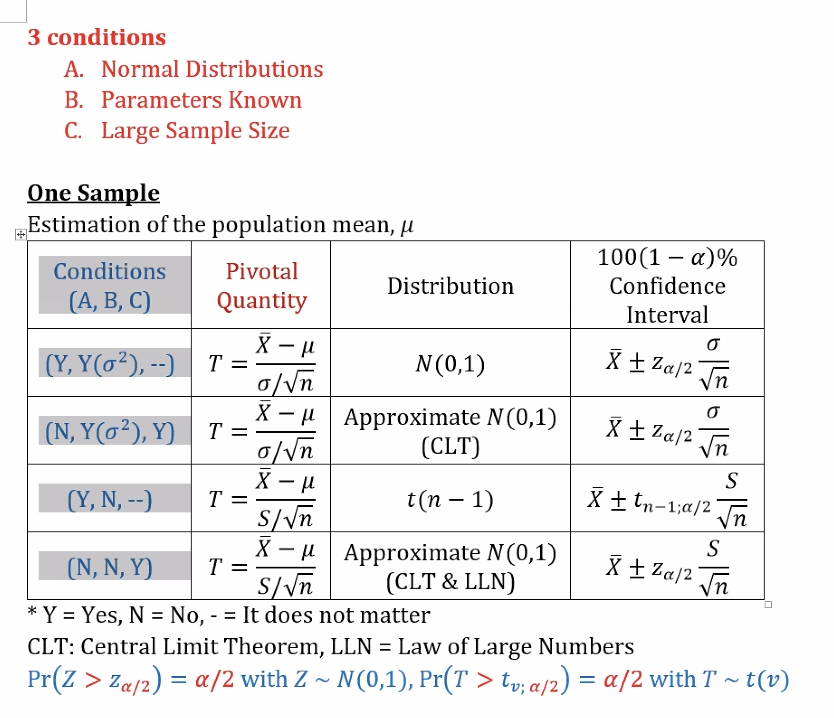
\includegraphics[width = 18cm]{Images/summary CI.png}
    \caption{Confidence Interval Summary}
    \label{fig:my_label}
\end{figure}
\begin{figure}[h]
    \centering
    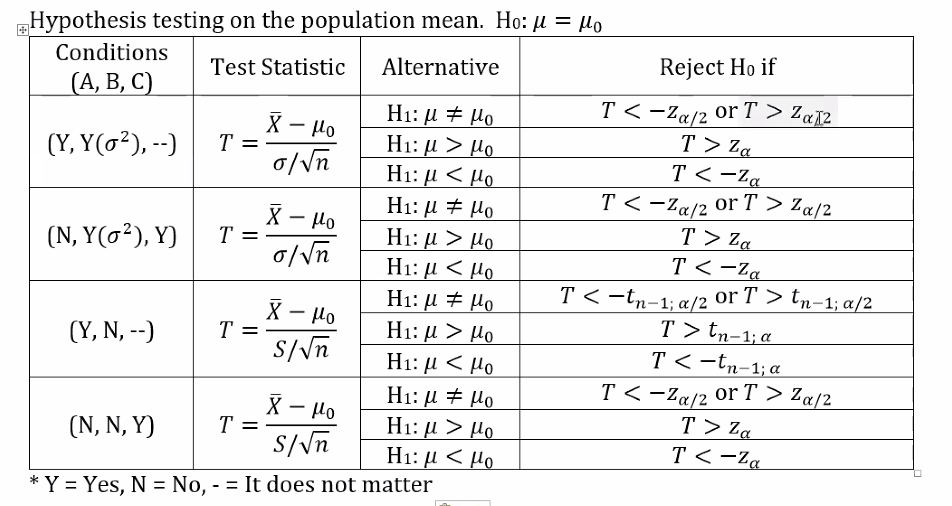
\includegraphics[width = 18cm]{Images/summary HT.png}
    \caption{Hypothesis Testing Summary}
    \label{fig:my_label}
\end{figure}